
\documentclass[letterpaper,hide notes,xcolor={table,svgnames},pdftex,10pt]{beamer}
\def\showexamples{t}

\usecolortheme{crane}
\setbeamertemplate{navigation symbols}{}

\usetheme{MyPittsburgh}
\usepackage{hyperref}
\usepackage{graphicx,xspace}
\usepackage[normalem]{ulem}
\usepackage{multicol}
\usepackage{amsmath,amssymb,amsthm,graphicx,xspace}
\newcommand\SF[1]{$\bigstar$\footnote{SF: #1}}

\usepackage[sfdefault,lf]{carlito}
\usepackage[T1]{fontenc}
\usepackage[scaled]{beramono}
\usepackage{tikzpagenodes}
\newcommand{\Rplus}{\protect\hspace{-.1em}\protect\raisebox{.35ex}{\small{\small\textbf{+}}}}
\newcommand{\Cpp}{\mbox{C\Rplus\Rplus}\xspace}

\newcounter{tmpnumSlide}
\newcounter{tmpnumNote}

\newcommand\mnote[1]{%
	\addtocounter{tmpnumSlide}{1}
	\ifdefined\showcues {~\tiny\fbox{\arabic{tmpnumSlide}}}\fi
	\note{\setlength{\parskip}{1ex}\addtocounter{tmpnumNote}{1}\textbf{\Large \arabic{tmpnumNote}:} {#1\par}}}

\newcommand\mmnote[1]{\note{\setlength{\parskip}{1ex}#1\par}}


\newcommand\mquestion[2]{{~\color{red}\fbox{?}}\note{\setlength{\parskip}{1ex}\par{\Large \textbf{?}} #1} \note{\setlength{\parskip}{1ex}\par{\Large \textbf{A}} #2\par}\ifdefined \presentationonly \pause \fi}

\newcommand\blackboard[1]{%
	\ifdefined   \showblackboard
		{#1}
	\else {\begin{center} \fbox{\colorbox{blue!30}{%
						\begin{minipage}{.95\linewidth}%
							\hspace{\stretch{1}} Some space intentionally left blank; done at the blackboard.%
						\end{minipage}}}\end{center}}%
	\fi%
}

\usepackage{listings}
\lstset{%
	keywordstyle=\bfseries,
	aboveskip=15pt,
	belowskip=15pt,
	captionpos=b,
	identifierstyle=\ttfamily,
	frame=lines,
	numbers=left, basicstyle=\scriptsize, numberstyle=\tiny, stepnumber=0, numbersep=2pt}

\usepackage{siunitx}
\newcommand\sius[1]{\num[group-separator = {,}]{#1}\si{\micro\second}}
\newcommand\sims[1]{\num[group-separator = {,}]{#1}\si{\milli\second}}
\newcommand\sins[1]{\num[group-separator = {,}]{#1}\si{\nano\second}}
\sisetup{group-separator = {,}, group-digits = true}

%% -------------------- tikz --------------------
\usepackage{tikz}
\usetikzlibrary{positioning}
\usetikzlibrary{arrows,backgrounds,automata,decorations.shapes,decorations.pathmorphing,decorations.markings,decorations.text}

\tikzstyle{place}=[circle,draw=blue!50,fill=blue!20,thick, inner sep=0pt,minimum size=6mm]
\tikzstyle{transition}=[rectangle,draw=black!50,fill=black!20,thick, inner sep=0pt,minimum size=4mm]

\tikzstyle{block}=[rectangle,draw=black, thick, inner sep=5pt]
\tikzstyle{bullet}=[circle,draw=black, fill=black, thin, inner sep=2pt]

\tikzstyle{pre}=[<-,shorten <=1pt,>=stealth',semithick]
\tikzstyle{post}=[->,shorten >=1pt,>=stealth',semithick]
\tikzstyle{bi}=[<->,shorten >=1pt,shorten <=1pt, >=stealth',semithick]

\tikzstyle{mut}=[-,>=stealth',semithick]

\tikzstyle{treereset}=[dashed,->, shorten >=1pt,>=stealth',thin]

\usepackage{ifmtarg}
\usepackage{xifthen}
\makeatletter
% new counter to now which frame it is within the sequence
\newcounter{multiframecounter}
% initialize buffer for previously used frame title
\gdef\lastframetitle{\textit{undefined}}
% new environment for a multi-frame
\newenvironment{multiframe}[1][]{%
	\ifthenelse{\isempty{#1}}{%
		% if no frame title was set via optional parameter,
		% only increase sequence counter by 1
		\addtocounter{multiframecounter}{1}%
	}{%
		% new frame title has been provided, thus
		% reset sequence counter to 1 and buffer frame title for later use
		\setcounter{multiframecounter}{1}%
		\gdef\lastframetitle{#1}%
	}%
	% start conventional frame environment and
	% automatically set frame title followed by sequence counter
	\begin{frame}%
		\frametitle{\lastframetitle~{\normalfont(\arabic{multiframecounter})}}%
		}{%
	\end{frame}%
}
\makeatother

\makeatletter
\newdimen\tu@tmpa%
\newdimen\ydiffl%
\newdimen\xdiffl%
\newcommand\ydiff[2]{%
	\coordinate (tmpnamea) at (#1);%
	\coordinate (tmpnameb) at (#2);%
	\pgfextracty{\tu@tmpa}{\pgfpointanchor{tmpnamea}{center}}%
	\pgfextracty{\ydiffl}{\pgfpointanchor{tmpnameb}{center}}%
	\advance\ydiffl by -\tu@tmpa%
}
\newcommand\xdiff[2]{%
	\coordinate (tmpnamea) at (#1);%
	\coordinate (tmpnameb) at (#2);%
	\pgfextractx{\tu@tmpa}{\pgfpointanchor{tmpnamea}{center}}%
	\pgfextractx{\xdiffl}{\pgfpointanchor{tmpnameb}{center}}%
	\advance\xdiffl by -\tu@tmpa%
}
\makeatother
\newcommand{\copyrightbox}[3][r]{%
	\begin{tikzpicture}%
		\node[inner sep=0pt,minimum size=2em](ciimage){#2};
		\usefont{OT1}{phv}{n}{n}\fontsize{4}{4}\selectfont
		\ydiff{ciimage.south}{ciimage.north}
		\xdiff{ciimage.west}{ciimage.east}
		\ifthenelse{\equal{#1}{r}}{%
			\node[inner sep=0pt,right=1ex of ciimage.south east,anchor=north west,rotate=90]%
			{\raggedleft\color{black!50}\parbox{\the\ydiffl}{\raggedright{}#3}};%
		}{%
			\ifthenelse{\equal{#1}{l}}{%
				\node[inner sep=0pt,right=1ex of ciimage.south west,anchor=south west,rotate=90]%
				{\raggedleft\color{black!50}\parbox{\the\ydiffl}{\raggedright{}#3}};%
			}{%
				\node[inner sep=0pt,below=1ex of ciimage.south west,anchor=north west]%
				{\raggedleft\color{black!50}\parbox{\the\xdiffl}{\raggedright{}#3}};%
			}
		}
	\end{tikzpicture}
}


%% --------------------

%\usepackage[excludeor]{everyhook}
%\PushPreHook{par}{\setbox0=\lastbox\llap{MUH}}\box0}

%\vspace*{\stretch{1}

%\setbox0=\lastbox \llap{\textbullet\enskip}\box0}

\setlength{\parskip}{\fill}

\newcommand\noskips{\setlength{\parskip}{1ex}}
\newcommand\doskips{\setlength{\parskip}{\fill}}

\newcommand\xx{\par\vspace*{\stretch{1}}\par}
\newcommand\xxs{\par\vspace*{2ex}\par}
\newcommand\tuple[1]{\langle #1 \rangle}
\newcommand\code[1]{{\sf \footnotesize #1}}
\newcommand\ex[1]{\uline{Example:} \ifdefined \presentationonly \pause \fi
	\ifdefined\showexamples#1\xspace\else{\uline{\hspace*{2cm}}}\fi}

\newcommand\ceil[1]{\lceil #1 \rceil}


\AtBeginSection[]
{
	\begin{frame}
		\frametitle{Outline}
		\tableofcontents[currentsection]
	\end{frame}
}



\pgfdeclarelayer{edgelayer}
\pgfdeclarelayer{nodelayer}
\pgfsetlayers{edgelayer,nodelayer,main}

\tikzstyle{none}=[inner sep=0pt]
\tikzstyle{rn}=[circle,fill=Red,draw=Black,line width=0.8 pt]
\tikzstyle{gn}=[circle,fill=Lime,draw=Black,line width=0.8 pt]
\tikzstyle{yn}=[circle,fill=Yellow,draw=Black,line width=0.8 pt]
\tikzstyle{empty}=[circle,fill=White,draw=Black]
\tikzstyle{bw} = [rectangle, draw, fill=blue!20,
text width=4em, text centered, rounded corners, minimum height=2em]

\newcommand{\CcNote}[1]{% longname
	This work is licensed under the \textit{Creative Commons #1 3.0 License}.%
}
\newcommand{\CcImageBy}[1]{%
	\includegraphics[scale=#1]{creative_commons/cc_by_30.pdf}%
}
\newcommand{\CcImageSa}[1]{%
	\includegraphics[scale=#1]{creative_commons/cc_sa_30.pdf}%
}
\newcommand{\CcImageNc}[1]{%
	\includegraphics[scale=#1]{creative_commons/cc_nc_30.pdf}%
}
\newcommand{\CcGroupBySa}[2]{% zoom, gap
	\CcImageBy{#1}\hspace*{#2}\CcImageNc{#1}\hspace*{#2}\CcImageSa{#1}%
}
\newcommand{\CcLongnameByNcSa}{Attribution-NonCommercial-ShareAlike}

\newenvironment{changemargin}[1]{% 
	\begin{list}{}{% 
		\setlength{\topsep}{0pt}% 
		\setlength{\leftmargin}{#1}% 
		\setlength{\rightmargin}{1em}
		\setlength{\listparindent}{\parindent}% 
		\setlength{\itemindent}{\parindent}% 
		      \setlength{\parsep}{\parskip}% 
		      }% 
		\item[]}{\end{list}}




\title{Lecture 23 --- File Allocation Methods }

\author{Jeff Zarnett \\ \small \texttt{jzarnett@uwaterloo.ca}}
\institute{Department of Electrical and Computer Engineering \\
  University of Waterloo}
\date{\today}


\begin{document}

\begin{frame}
  \titlepage

 \end{frame}


\begin{frame}
\frametitle{Allocation of Disk Space}

There is a need to choose a strategy for how to allocate disk space. 

\begin{center}
	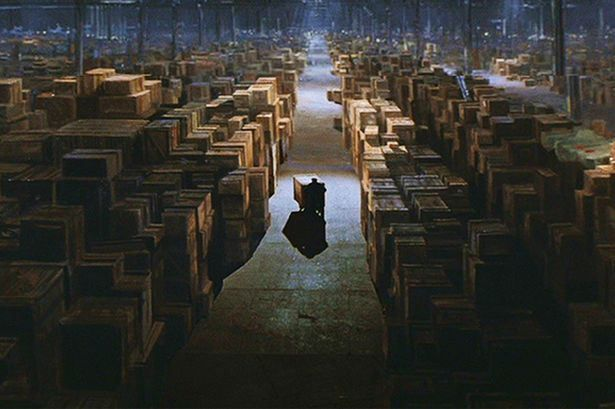
\includegraphics[width=0.4\textwidth]{images/jones.jpg}
\end{center}

There are three major ways that we could allocate the disk space to files:\\
\quad Contiguous, linked, and indexed; each has its advantages and disadvantages.


\end{frame}

\begin{frame}
\frametitle{Contiguous Allocation}
Contiguous: a file occupies a set of contiguous blocks on disk. 

So a file is allocated, starting at block $b$ and is $n$ blocks in size, the file takes up blocks $b, b+1, b+2, ..., b+(n-1)$. 

This is advantageous, because if we want to access block $b$ on disk, accessing $b+1$ requires no head movement, so seek time is nonexistent to minimal.

\end{frame}

\begin{frame}
\frametitle{Contiguous Allocation}

All that we need to maintain are $b$ and $n$: the start location and length of the file. 

Both sequential and direct access are very easy: the first block of a file is at $b$. 

To access a block $i$ at some offset into the file, it's at the base address $b$ plus $i$. 

Checking if the access is valid is also an easy operation: if $i < n$ then it is valid.

\end{frame}

\begin{frame}
\frametitle{Contiguous Allocation}

\begin{center}
	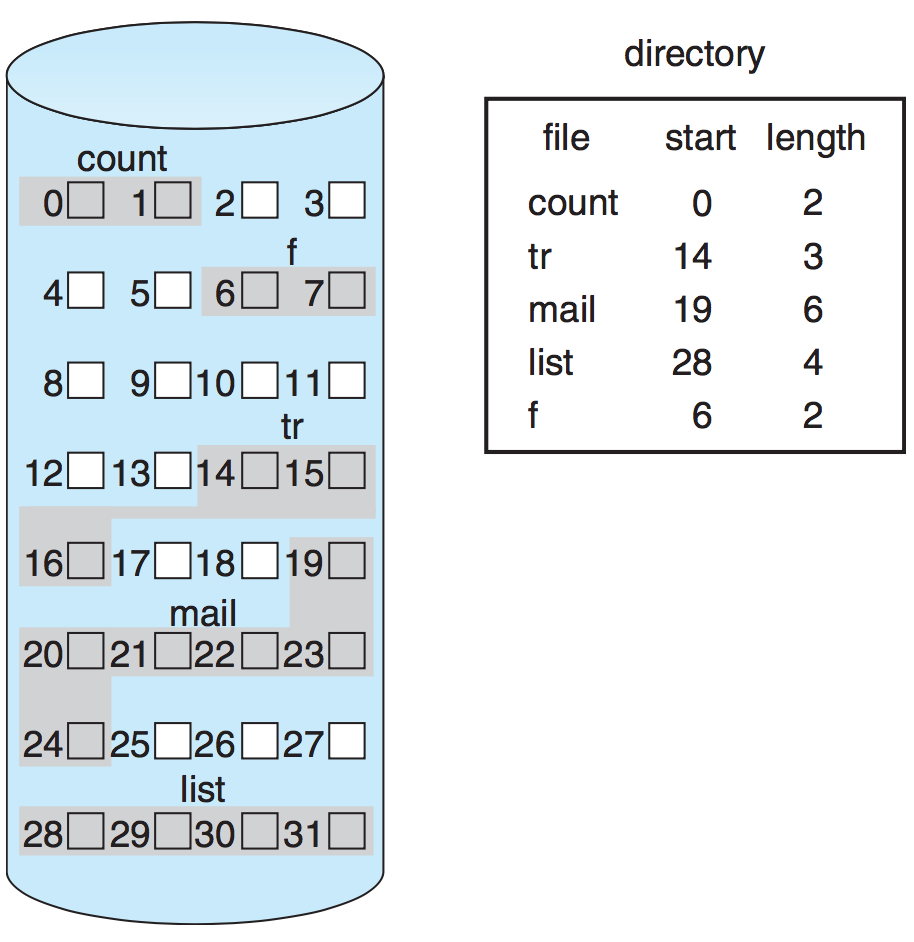
\includegraphics[width=0.6\textwidth]{images/disk-contiguous.png}
\end{center}

\end{frame}

\begin{frame}
\frametitle{Contiguous Allocation}

This takes us back to a problem we have seen once before: the memory allocation problem. 

If we need a memory block of size $N$:\\
\quad (1) can we find a contiguous block of $N$ or greater to meet that allocation?\\
\quad (2) if there is more than one block, which one do we choose? 

As before, we suffer the problem of external fragmentation, plus a bit of internal fragmentation in the last block of the file. 

\end{frame}

\begin{frame}
\frametitle{Contiguous Allocation and Compaction}

There was also talk on the subject of memory allocation of compaction. 

This was moving memory allocations around in memory to create some larger free spaces that can be allocated. 

But for languages like C, it was not realistic, because of the impossibility of updating all pointers (unlike Java where we can update all references). 

\end{frame}

\begin{frame}
\frametitle{Compaction}

We can do compaction on disk, but it's slow and computationally expensive. 

Doing compaction can be done when the system has nothing else to do (idle priority operation) or on some schedule when it would be minimally disruptive.

The middle of the night...?


\end{frame}

\begin{frame}
\frametitle{Contiguous Allocation}

Another problem: how much space is a file going to take? 

If it is just a copy-paste operation, the copy is the same size as the original. 

When a user opens a new document, how big will it be? 

\end{frame}

\begin{frame}
\frametitle{Contiguous Allocation}


If we allocate too little space, we may be able to tack on space at the end, or that block may be allocated, forcing us to move the file and reallocate it. 

If the value we choose is too large, then significant space will be wasted for small files (and many files tend to be relatively small).

\end{frame}

\begin{frame}
\frametitle{Linked Allocation}

Linked allocation is a solution to the problems of contiguous allocation.

Instead of a file being all in consecutive blocks, we maintain a linked list of the blocks, and the blocks themselves may be located anywhere on the disk. 

The directory listing just has a pointer to the first and last blocks (head and tail of the linked list).

\end{frame}

\begin{frame}
\frametitle{Linked Allocation}

If a new file is created, it will be created with size zero and the head and tail pointers are null.

 When a new block is needed, it can come from anywhere and will just be added to the linked list. 
 
 Thus, compaction and relocation are not really an issue. 
 
 Unfortunately, however, accessing block $i$ of a file is no longer as simple as computing an offset from the first block; it requires following $i$ pointers (a pain).


\end{frame}

\begin{frame}
\frametitle{Linked Allocation}

\begin{center}
	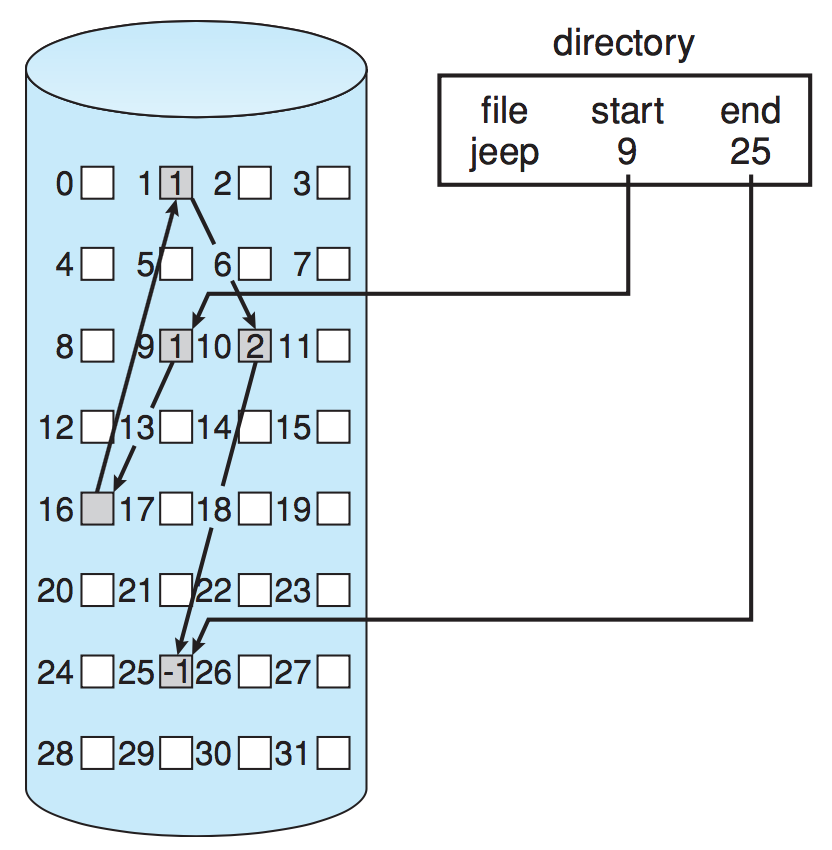
\includegraphics[width=0.6\textwidth]{images/disk-linked.png}
\end{center}

\end{frame}

\begin{frame}
\frametitle{Linked Allocation}

A possible solution to the problem of following so many pointers (and the overhead of maintaining so many) is to group up the blocks into \alert{clusters}.

A cluster is comprised of, say, four blocks. 

Then we waste less memory maintaining pointers and it improves disk accesses because there is less seeking back and forth to various disk locations.

\end{frame}

\begin{frame}
\frametitle{File Allocation Table (FAT)}

One variation of linked allocation is the File Allocation Table (FAT).

Used in Windows before NTFS came in with Windows NT/2000/XP/7/8...

FAT32 hangs on these days for USB Flash Drives.

\end{frame}

\begin{frame}
\frametitle{File Allocation Table}


At the beginning of the disk, there is a table to maintain file allocation data. 

The table has one entry for each block and is indexed by block number. 

It works like a linked list; the directory entry has the first block of the file and the table entry under that block number has the index of the next block. 

The chain continues until the last block; there is a special end-of-file value. 

\end{frame}

\begin{frame}
\frametitle{File Allocation Table}

An unused block has a table value of 0. 

Thus, to allocate a new block, find the first 0-valued entry, and replace the previous end-of-file value with the address of the new block.

\end{frame}

\begin{frame}
\frametitle{File Allocation Table}

\begin{center}
	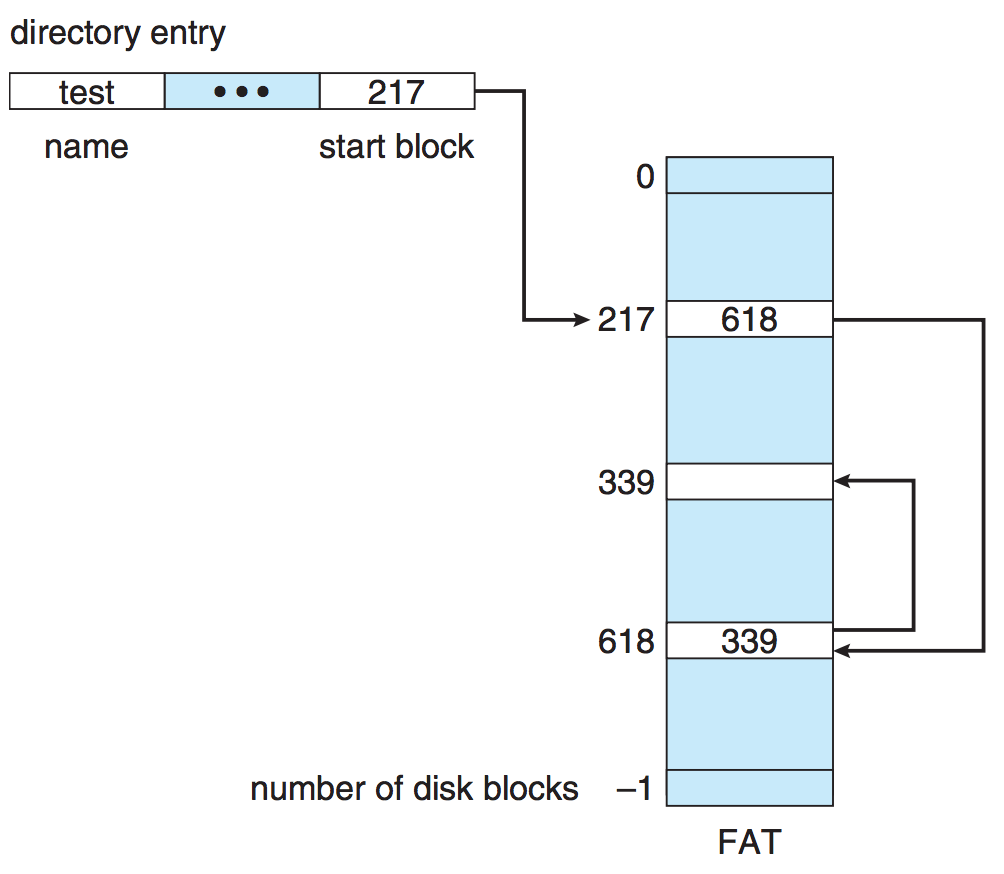
\includegraphics[width=0.6\textwidth]{images/file-allocation-table.png}
\end{center}

The FAT itself should be cached in memory, otherwise the disk is going to have to seek back to it unbearably often.

\end{frame}



\begin{frame}
\frametitle{Indexed Allocation}

If we stuck to pure linked allocation, we still have the problem that accessing some part in the middle of the file is a pain.

We have to follow and retrieve a lot of pointers to the different blocks. 

The idea of indexed allocation is to take all the pointers and put them into one location: an index block. 


\end{frame}



\begin{frame}
\frametitle{Indexed Allocation}

So, the first block of the file contains a whole bunch of pointers. 

To get to block $i$, just go to index $i$ of the index block and we can get the location of block $i$ much more efficiently than we could in linked allocation. 

All pointers to blocks start as null, and when we add a new block, add its corresponding entry into the index block.

\end{frame}

\begin{frame}
\frametitle{Indexed Allocation}

\begin{center}
	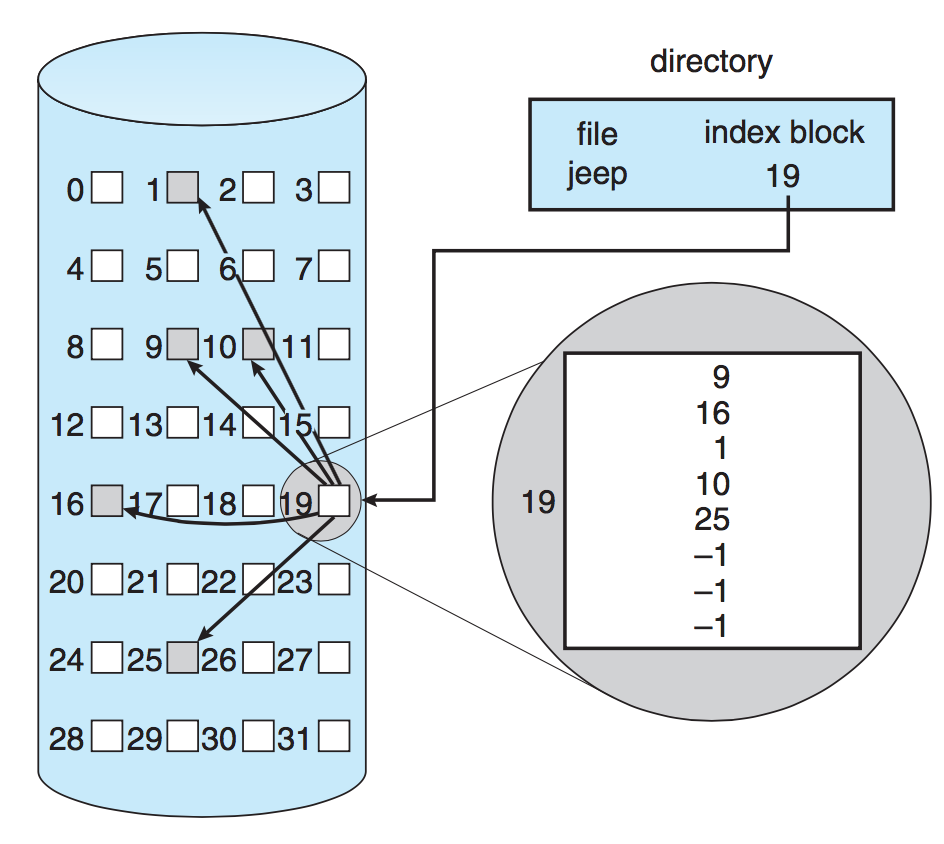
\includegraphics[width=0.6\textwidth]{images/disk-indexed.png}
\end{center}


\end{frame}

\begin{frame}
\frametitle{Block Size}

Like many of the other systems we have examined, there is a need to make a decision about the size of a block. 

If a file needs only 1-2 blocks, one whole block is allocated for the pointers which contains only 1-2 entries. 

That suggests we want the index to be small, but what if we need more pointers than fit into one block? There are a few mechanisms for this.


\end{frame}

\begin{frame}
\frametitle{Block Size}

What if we need more pointers than fit into one block?

\begin{enumerate}
	\item \textbf{Linked Scheme}
	\item \textbf{Multilevel Index}
	\item \textbf{Combined Scheme}
\end{enumerate}


\end{frame}

\begin{frame}
\frametitle{UNIX inodes}

We can finally show a visual representation of an inode.

\begin{center}
	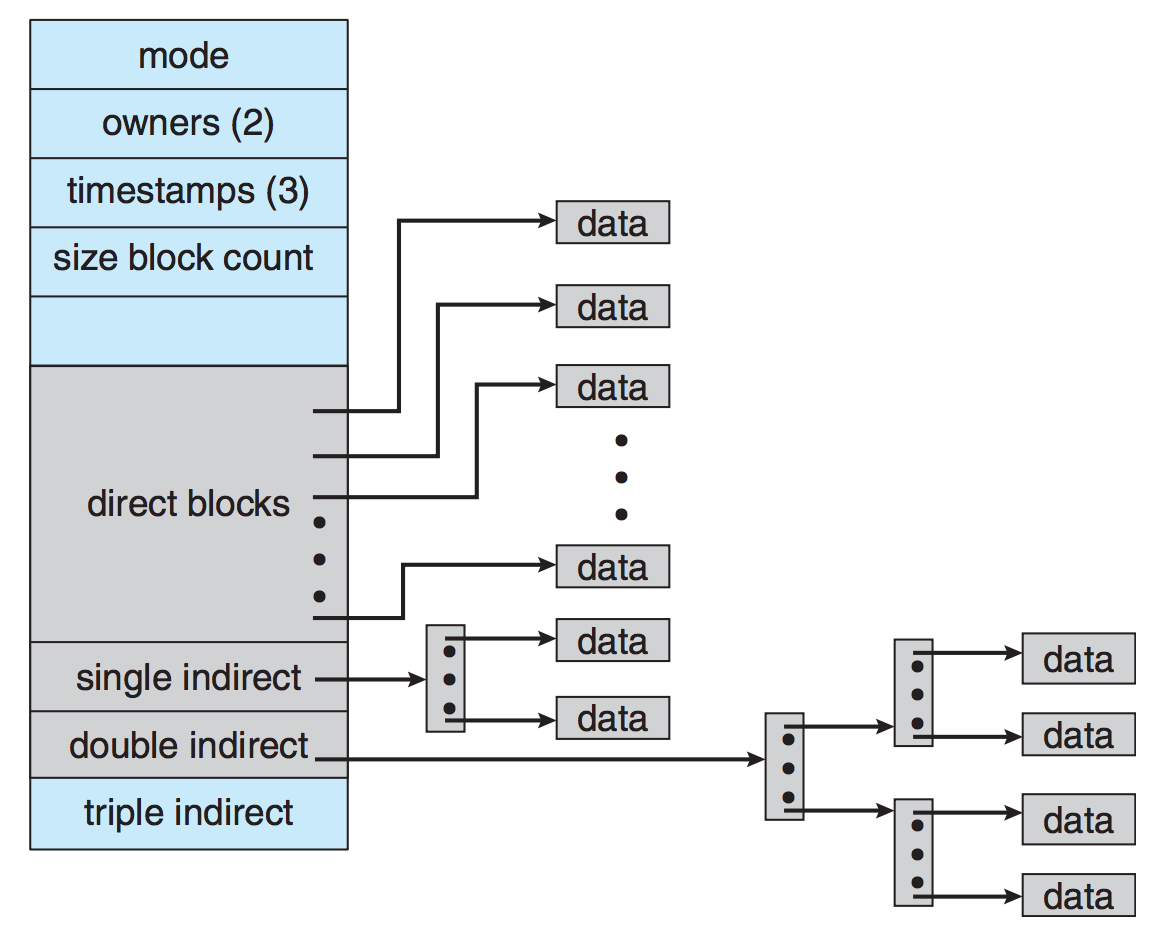
\includegraphics[width=0.6\textwidth]{images/unix-inode.png}
\end{center}


\end{frame}

\begin{frame}
\frametitle{Free Space Management}

As with memory, the system will keep track of the free space available.

Bit vectors work just the way we would expect: create a structure in memory where a bit represents a block. 

If it is free, the bit is 1; allocated is 0. 

So a bit vector looks like \texttt{0100110111011111000000...}. 

The problem with this strategy is, of course, that the bigger the disk, the more overhead is needed to store this bit vector.

\end{frame}

\begin{frame}
\frametitle{Free Space Management}

The next rather obvious approach is a linked list: the head points to the first free space block, and we can traverse the list to get to the next free block. 

\begin{center}
	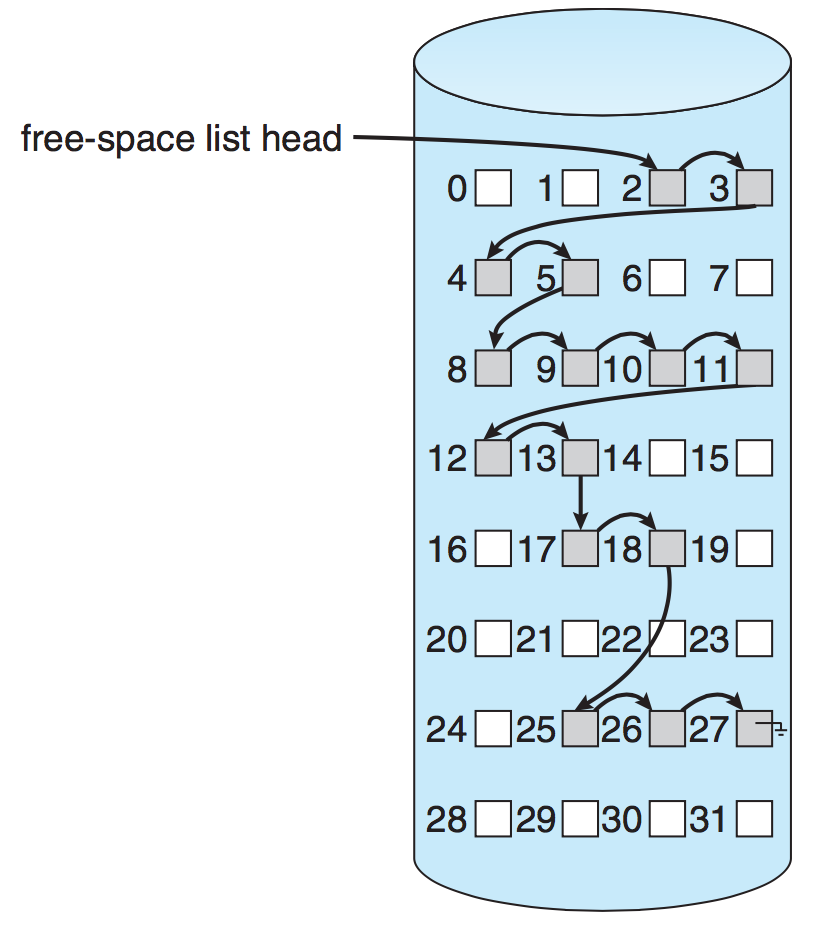
\includegraphics[width=0.4\textwidth]{images/disk-linked-list.png}
\end{center}


\end{frame}

\begin{frame}
\frametitle{Grouping}

Grouping: the first free block will be used to store the addresses of $n$ free blocks, the first $n-1$ of which are actually free. 

The last block contains a block with another set of $n$ free blocks. 

So if we need a large number of free blocks, we can find them quickly, instead of walking through the list one block at a time, which takes a lot of disk accesses. 

\end{frame}

\begin{frame}
\frametitle{Counting}

Counting is a slight improvement on this where we also store a number $k$ of free contiguous blocks after each address. 

So, if block 27 is followed by three consecutive free blocks, instead of having 27, 28, 29, 30 as entries, it will show (27, 4). 

The entries may be stored in a balanced tree for efficient operations.~



\end{frame}

\begin{frame}
\frametitle{Preallocation}

The efficient use of a disk depends on the disk-allocation/directory algorithms. 

UNIX inodes, for example, are preallocated, so even a disk containing no files has some of its space taken up by the inodes. 

Preallocation \& distribution of inodes improves the file system performance.

UNIX allocation and free-space algorithms keep the file data near the inode, where possible, to reduce seek time.


\end{frame}

\begin{frame}
\frametitle{Consistency Checking and Journalling}

Unfortunately, an error, crash, or power failure or something similar may result in a loss of data or inconsistent data in the file system. 

The directory structures, pointers, inodes, FCBs, et cetera are all data structures and if they become corrupted it may lead to serious problems.


\end{frame}

\begin{frame}
\frametitle{Consistency Checking}

We could check for inconsistent data periodically (e.g., on system boot up) and many operating systems do so. 

This is, of course, an operation that will consume a very large amount of time while the whole disk is scanned. 

UNIX: \texttt{fsck}. Windows: \texttt{chkdsk}/\texttt{scandisk}.

\begin{center}
	
\includegraphics[width=0.3\textwidth]{images/swearwords.jpg}
\end{center}

\end{frame}

\begin{frame}
\frametitle{Consistency Checking}

These tools will look for inconsistent states (e.g., a file that claims to be 12 blocks but the linked list contains only 5) and will attempt to repair it.

Its level of success depends on the nature of the problem and the implementation of the file system.

\end{frame}



\begin{frame}
\frametitle{Preventing the Problem}

Obviously we would like to prevent the problem, if we can. 

Atomic operations: an operation should either succeed completely, or not take place at all. 

This approach is used in the Windows NTFS system as well as Mac OS HFS+.


\end{frame}

\begin{frame}
\frametitle{Transactions}

We might be familiar, at this point, with the concept of the \alert{transaction}.

Before making any changes, make a list of all the things we plan to do. 

Then do the things written down. 

Then we consider the transaction complete.

\end{frame}

\begin{frame}
\frametitle{Transactions}

All metadata changes are written sequentially to a log file; once the changes are written to the log, control returns to the program that requested the operation. 

Meanwhile, the log entries are actually carried out. 

As changes are made, a pointer is updated to indicate which of the log entries have really happened and which have not.

When an entire transaction is completed, it is removed from the log file. If the system crashes, the log file will contain zero or more transactions.
\end{frame}

\begin{frame}
\frametitle{Transactions}

If zero, there is no problem: nothing was in progress at the time of the crash. 

If there are some, then the transactions were not completed and the operations should still be carried out. 

If a transaction was aborted (not committed), we walk backwards through the log entries to undo any completed operations.

Thus, we go back to the state before the start of the transaction.




\end{frame}

\begin{frame}
\frametitle{Data Loss}

Even though a particular write may not have taken place because of a crash, resulting in some data loss, the system will always remain in a consistent state. 

As a side benefit, we can sometimes re-order the writes to get better performance (e.g., schedule them to get better disk utilization). 


\end{frame}

\begin{frame}
\frametitle{ZFS Approach}

The approach in the Solaris ZFS approach is similar, but not identical. 

Blocks are never overwritten with new data.\\
\quad Instead, a transaction writes all data and metadata to new blocks. 

Only when the transaction is complete, any references to the old blocks are replaced with the location of the new blocks. 


Then the old pointers and blocks can be cleaned up (reused or disposed of). 


\end{frame}



\begin{frame}
\frametitle{Example: NTFS (Windows File System)}

NTFS uses several different storage levels:

\begin{enumerate}
	\item \textbf{Sector}
	\item \textbf{Cluster}
	\item \textbf{Volume}
\end{enumerate}


\end{frame}

\begin{frame}
\frametitle{NTFS}

The cluster is the fundamental unit of allocation of NTFS.

This allows the file system to be independent of the size of physical sectors on the disk. 

A volume contains file system information, a collection of files, and free space. 

The logical volume may be some of a physical disk, all of one, or spread across multiple physical disks.

\end{frame}

\begin{frame}
\frametitle{NTFS Volume Layout}

\begin{center}
	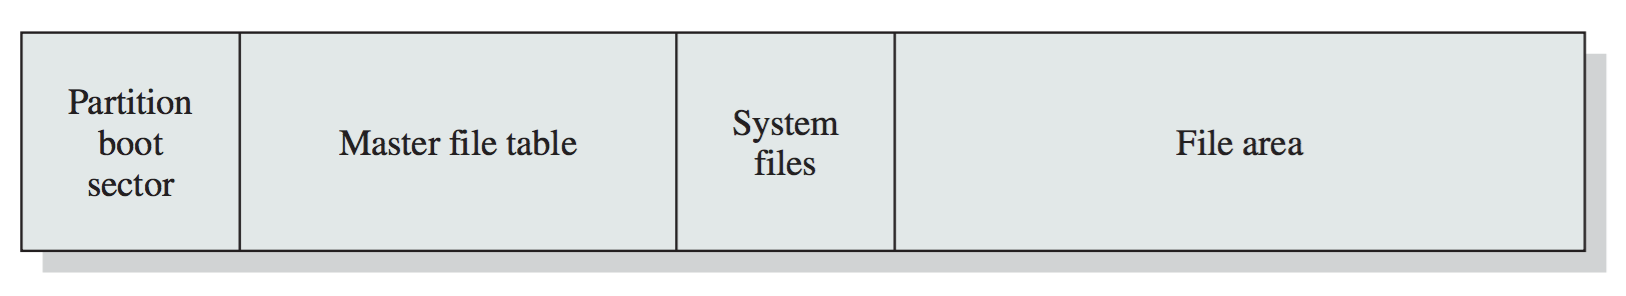
\includegraphics[width=0.9\textwidth]{images/ntfs-volume.png}
\end{center}

\end{frame}

\begin{frame}
\frametitle{NTFS System Files}

The Master File Table (MFT) contains information about all the files and folders. 

A block is allocated to system files that contain important system information:

\begin{enumerate}
	\item \textbf{MFT2}
	\item \textbf{Log File}
	\item \textbf{Cluster Bitmap}
	\item \textbf{Attribute Definition Table}
\end{enumerate}
\end{frame}



\begin{frame}
\frametitle{NTFS File and Directory Attributes}

\begin{center}
	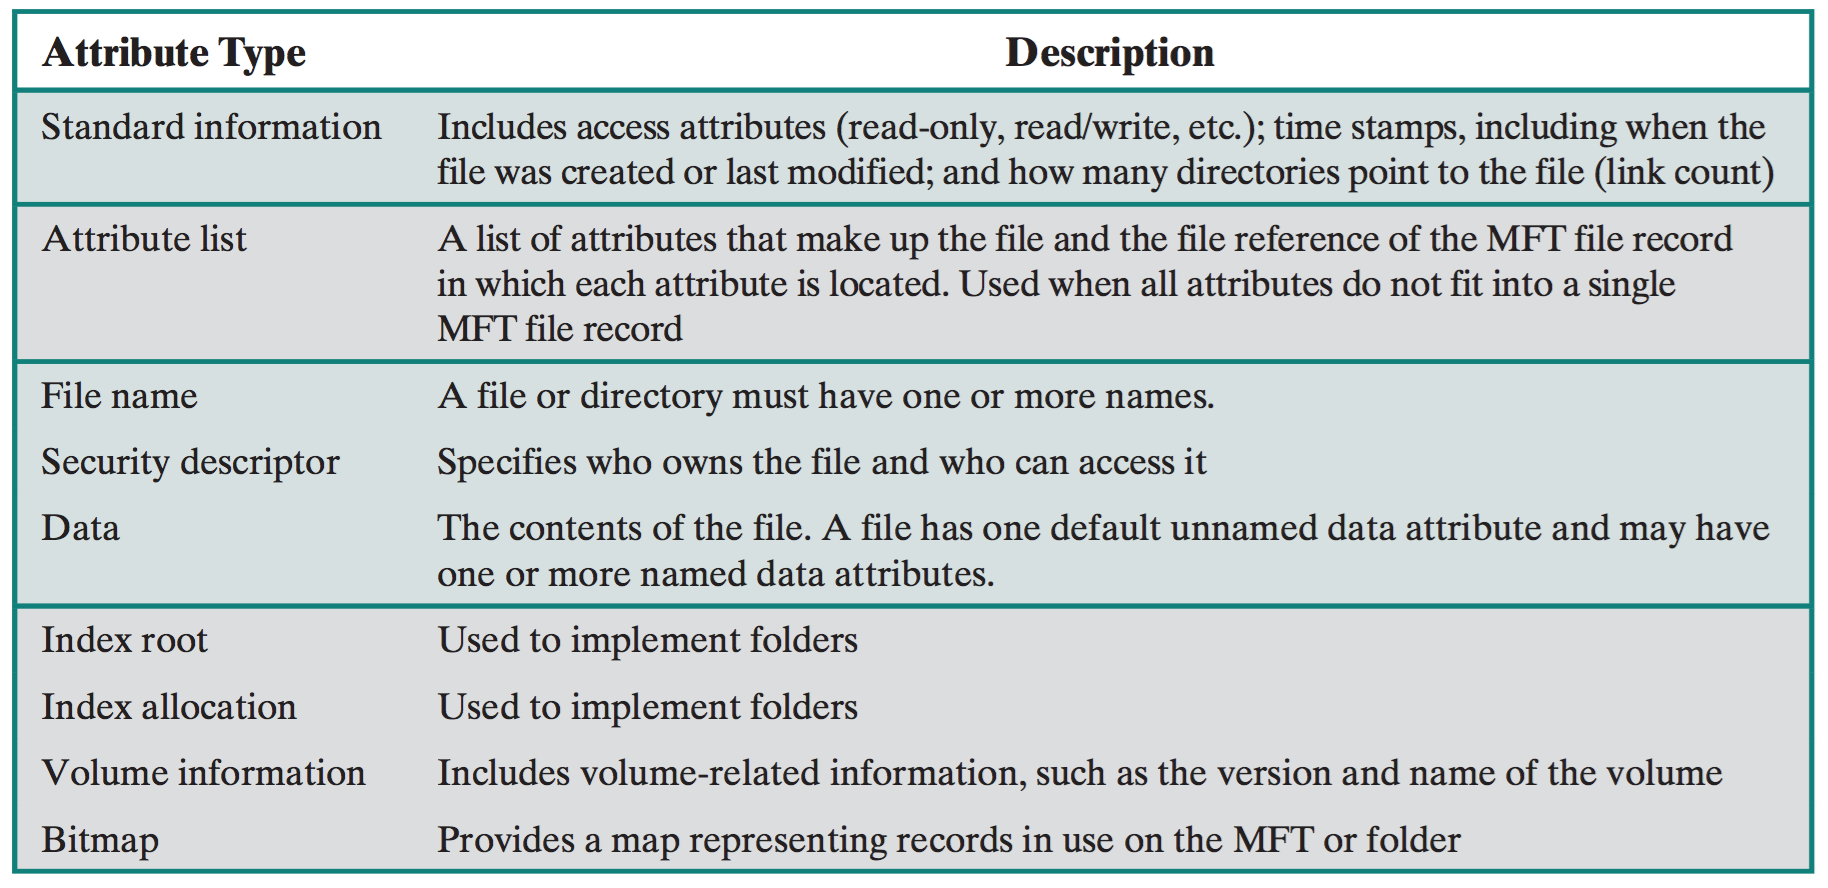
\includegraphics[width=\textwidth]{images/ntfs-attrs.png}
\end{center}


\end{frame}

\begin{frame}
\frametitle{NTFS Journalling}

NTFS uses journalling to ensure that the file system will be in a consistent state at all times, even after a crash or restart. 

There is a service responsible for maintaining a log file that will be used to recover in the event that things go wrong.  

Note that the goal of recovery is to make sure the system-maintained metadata is in a consistent state; user data can still get lost. 

This was a Microsoft design decision.


\end{frame}

\begin{frame}
\frametitle{NTFS Journalling Implementation}

The actual implementation of journalling:

\begin{enumerate}
	\item Record the change(s) in the log file in the cache.
	\item Modify the volume in the cache.
	\item The cache manager flushes the log file to disk.
	\item Only after the log file is flushed to disk, the cache manager flushes the volume changes.
\end{enumerate}

\end{frame}

\begin{frame}
\frametitle{Backups}

We often think of them as places for permanent storage of data, but hard drives can and do fail. 


\begin{center}
	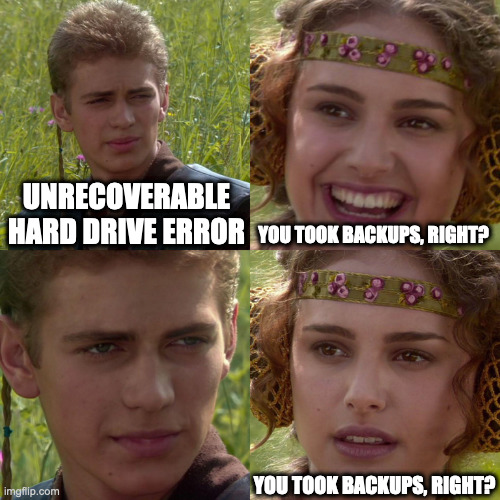
\includegraphics[width=0.5\textwidth]{images/backups.jpg}
\end{center}

So please, take backups of important data.


\end{frame}

\end{document}

